\documentclass[a0,portrait]{a0poster}
%\usepackage{alltt}
\usepackage{color}
\usepackage{times}
\usepackage{amsmath,amsfonts,amssymb} % God matematik
\usepackage{a0poster}
\usepackage{pst-node,graphicx}
\usepackage[utf8]{inputenc} % ÆØÅ pakken
\usepackage[T1]{fontenc}
%\usepackage[pdftex,bookmarks=true,bookmarksnumbered=true]{hyperref}

%%%%%%%%%%%%%%%%%%%%%%%%%%%%%%%%%%%%%%%%%%%%%%%%%%%%%%%%%%%%%%%%%%%%%%%%%%%%%


\begin{document}
\title{Centralized State Estimation of Distributed Maritime} % Line one of the title
\titletwo{Autonomous Surface Oceanographers} % Line two of the title.
\author{Rasmus L. Christensen, Federik Juul, Nick \O stergaard, Tudor Muresan, Attila Fodor}
\address{Section for Control and Automation, Department of Electronic Systmes, Aalborg University, Denmark$^\dagger$}
\email{\{ralch,nickoe,fjuul,tudor,attila\}@es.aau.dk}

\makeheader
%% Column 1
\begin{center}
\col{
\paragraph{Introduction}
Greenland has in excess of 30.000 kilometers of coastal line with outdated maps. This poses a danger as cruise ships currently navigate these waters carrying as many as 5000 passengers. If such a ship were to hit a rock and capsize, the nearest rescue station along the eastern coast of Greenland can be as many as 1000 kilometers away, and the infrastructure in these areas are not able to handle such a disaster. Therefore a fast, inexpensive and reliable solution to measuring the coast line will be developed throughout this project? (the last sentence is stupid..). 
\paragraph{Problem}
Jeepers. 

\paragraph{Path Optimization}
The path planner divides the path into straight and turning subsegments. The interesting part of this, is the turning subsegments. The turning segments are each defined by a threshold $\varepsilon_\text{max}$ which defines which algorithm to use dependent on the curvature of the path. The sub-waypoints are computed using the normalized Fresnel integral functions $C_F$ and $S_F$ in equation (\ref{eq:fresnel}) generating an Euler spiral in and out of the turn. 
\begin{align}
C_F(x) = \int_0^x \cos(t^2)dt,\,\,\,\,S_F(x) = \int_0^x \sin(t^2)dt
\label{eq:fresnel}
\end{align}
This allows for the ship to keep as much momentum as possible. If the curvature is below the threshold $\varepsilon < \varepsilon_\text{max}$ the algorithm only computes 3 key sub-waypoints as seen on figure \ref{fig:3points}:
\begin{figure}
	\centering % Figure input
	\includegraphics[width=\threecolwidth]{img/3points}
  	\caption{Sub waypoint calculation when $\varepsilon < \varepsilon_\text{max}$}
	\label{fig:3points}
\end{figure}
These waypoints are generated using the following calculations:
\begin{align}
A_3 = (-X_1,Y_1),\, C_3 = (0,\frac{y_d}{cos(\varepsilon)}),\, E_3 = (X_1,Y_1)
\end{align}
$X_1$ and $Y_1$ are calculated by:
\begin{align}
X_1 = x_d \cdot \cos(\varepsilon) + y_d \cdot \sin(\varepsilon),\,\,\,\, Y_1 = X_1 \cdot 	\tan(\varepsilon)
\end{align}
$x_d$ and $y_d$ are the variables calculated by the normalized Fresnel integrals, and contains the factor $\eta$ that allows the ship to preserve energy whilst turning:
\begin{align}
x_d = \frac{\pi}{\eta}\cdot C_F(\varepsilon),\,\,\, y_d = \frac{\pi}{\eta}\cdot S_F(\varepsilon),\,\,\, \eta = \frac{\text{max}\{\dot{\alpha}\}}{v^2}
\end{align}
Where $\dot{\alpha}$ is the amount of jerk the ship experiences when turning. If however the angle is above the threshold, $\varepsilon > \varepsilon_\text{max}$ more waypoints are added, and the coordinates become as seen on figure \ref{fig:5points}:
\begin{figure}
	\centering % Figure input
	\includegraphics[width=\threecolwidth]{img/5points}
  	\caption{Something}
	\label{fig:5points}
\end{figure}
More sub-waypoints are added to the system if a tighter path curvature is required, thus allowing the ship to still maintain its momentum:
\begin{align}
A_5 &= (-X_1,Y_1),\, B_5 = (-X_2,Y_2),\, C_5 = (0,Y_R)\\
D_5 &= (X_2,Y_2),\, E_5 = (X_1,Y_1)
\end{align}


}
%% Column 2
\rput{Center}{
\includegraphics[width=1.9\textwidth]{img/background.pdf}} % Background image
\col{
\paragraph{}
The computation of these 5 sub-waypoints are carried out as follows:
\begin{align}
X_R &= R_\text{min} \cdot \sin(\varepsilon - \varepsilon _\text{max}),\,\, P_X = X_R + y_d \cdot \sin(\varepsilon)\\
X_1 &= P_X + x_d \cdot \cos(\varepsilon),\,\, Y_1 = X_1 \cdot \tan(\varepsilon)\\
P_Y &= Y_1 - x_d \cdot \sin(\varepsilon),\,\, Y_2 = P_Y + y_d \cdot \cos(\varepsilon)\\
O_Y &= R_\text{min} \cdot \cos(\varepsilon - \varepsilon _\text{max}) + Y_2,\,\, R_Y = O_Y - R_\text{min}\\
X_2 &= X_R
\end{align}
The above computes the optimal path for the ship to follow as well as one where it preserves as much energy as possible whilst sailing it. 

\paragraph{Ship model}
To develop a control algorithm to carry out the inputs computed by the path planning algorithm, a low-level controller is developed. This is based around the 3 degree-of-freedom state model developed for the ship. The state model has been derived to be: \cite{sorensen}:
\begin{align}
\dot{\begin{bmatrix}
v\\
\theta\\
\omega
\end{bmatrix}} = \begin{bmatrix}
\frac{-\beta_x}{m} & 0 & 0\\
0 & 0 & 1\\
0 & 0 & \frac{-\beta_\omega}{I}
\end{bmatrix}\begin{bmatrix}
v\\
\theta\\
\omega
\end{bmatrix} + \begin{bmatrix}
\frac{1}{m} & 0\\
0 & 0\\
0 & \frac{1}{I}
\end{bmatrix}\begin{bmatrix}
F\\
\tau
\end{bmatrix}
\end{align}
$\beta_x$ and $\beta_\omega$ are the linearized skin frictional drag the ship expriences as it moves through the water. $F$ and $\tau$ are the forward force input and the torque generated by the difference in propeller revolutions. The discrete version of this is computed using the zero-order hold algorithm. The low-level control is carried out by reference tracking and optimal feedback control. 

\paragraph{State estimation}
To further improve the amount of 
The state model for the Kalman filter computed to be - which 
\begin{align}
\vec{\Phi} = diag\{\vec{\Phi} _x,\vec{\Phi} _y,\vec{\Phi} _\omega\},\,\, \vec{\Phi}_{x,y,\omega}(k) = \begin{bmatrix}
1 & t_s & \frac{t_s^2}{2}\\
0 & 1 & t_s\\
0 & \frac{-\beta_{x,y,\omega}}{m} & 0
\end{bmatrix}
\end{align}

As the radio link does not contain any redundancy, a lost packet will be handled by the Kalman filter, by reducing the gain of the filter to zero. If packet verification fails, the filter uses a gain mask $\vec{\Lambda}$ to zero the gains. This mask is post multiplied onto the Kalman gain $\bar{\vec{K}}$ and is defined as:
\begin{align}
\vec{\Lambda} = diag\{\lambda_x,\lambda_{\dot{x}},\lambda_{\ddot{x}},\lambda_{\lambda{y}},\lambda_{\dot{y}},\lambda_{\ddot{y}},\lambda_{\theta},\lambda_{\omega},\lambda_{\alpha} \}
\end{align}
Where the individual $\lambda$s are given as:
\begin{align}
\lambda = 
\left\{
  \begin{array}{l l}
    1 & \quad \text{if measurement is valid}\\
    0 & \quad \text{otherwise}
  \end{array} \right.
\end{align} 
The filter also needs to sort out the different sampling rate aboard the ship. The two main sensors, IMU and GPS, sample at 10 Hz and 1 Hz respectively - which also defines a mask to multiply onto the Kalman filter. This mask puts the gain to zero for the GPS if there is no new sample available. Figure \ref{fig:trends} depicts the absolute error between the true and estimated path for the 3 cases described above.

As the filter only needs to estimate 3 states, 


}
%% Column 3
\col{
\paragraph{}
\begin{figure}
	\centering % Figure input
	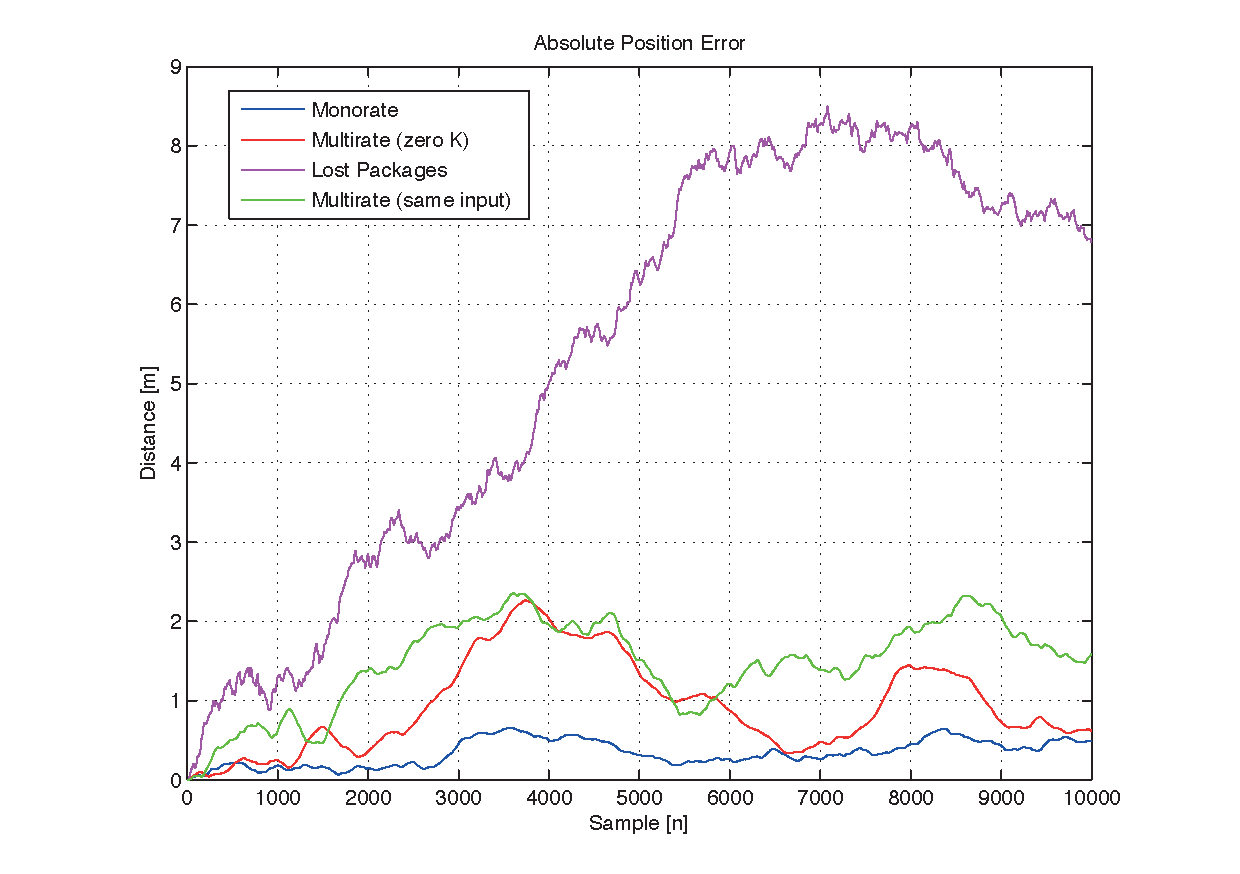
\includegraphics[width=\threecolwidth]{img/10percent}
  	\caption{Simulation of the system where the blue represents a mono-rate filter, the red a filter with zero-gaining when no measurements are available, the green where no zero-gaining takes place, and finally the purple where there is a 10 percent loss rate on the Kalman filter.}
	\label{fig:trends}
\end{figure}
\paragraph{Results}
Results on lost packages. 
\paragraph{Further results}
Something else?
\paragraph{Conclusion and extensions}
We can from this conclude that there is a problem.
\paragraph{Acknowledgements} A big thanks should be extended to Assistant Professor Carles Navarro Manchón for his help with tuning the Kalman filter. 

\references
\bibliography{litterature}
}
\end{center}

\makefooter
\end{document}





